\documentclass[border=4pt]{standalone}
% Shared typography and colours for the standalone figures.
\usepackage{unicode-math}
\setmainfont{TeX Gyre Termes}
\setmathfont{TeX Gyre Termes Math}
\usepackage{tikz}
\usetikzlibrary{arrows.meta,positioning,calc,decorations.pathreplacing}
\usepackage{pgfplots}
\pgfplotsset{compat=1.18}

% One colour per element or subsystem. Record the mapping in
% the working repository conventions and use it identically in every figure.
\definecolor{elemA}{HTML}{1F5FA8}
\definecolor{elemB}{HTML}{B8461B}
\definecolor{elemC}{HTML}{2E7D32}
\definecolor{elemD}{HTML}{6A4C93}
\definecolor{frameline}{HTML}{555555}

% Article-specific diagram styling; common figure-style.tex remains managed.
\usepackage{circuitikz}
\usetikzlibrary{decorations.pathmorphing,fit,backgrounds}
\tikzset{
  every node/.style={font=\small},
  block/.style={draw=frameline,rounded corners=2pt,minimum height=7mm,align=center,fill=white},
  massA/.style={draw=elemA,fill=elemA!10,thick},
  massB/.style={draw=elemB,fill=elemB!10,thick},
  receiver/.style={draw=elemC,fill=elemC!9,thick},
  mediator/.style={draw=elemD,fill=elemD!8,thick},
  flow/.style={-{Latex[length=2.3mm]},thick},
  boundary/.style={draw=frameline,dashed,rounded corners=3pt},
  spring/.style={decorate,decoration={coil,aspect=.4,segment length=3mm,amplitude=1.5mm},thick,elemD}
}

\begin{document}
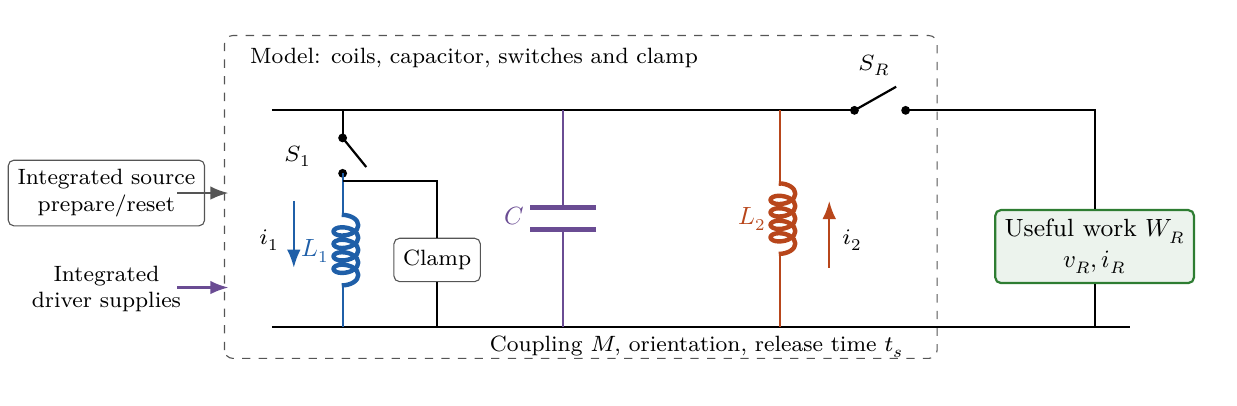
\begin{tikzpicture}
\path[use as bounding box] (0,-.65) rectangle (15,3.8);
\draw[boundary] (2.5,-.4) rectangle (11.55,3.7);
\node[font=\footnotesize,anchor=north west] at (2.7,3.67) {Model: coils, capacitor, switches and clamp};
\draw[thick] (3.1,2.75)--(10.5,2.75);
\draw[thick] (3.1,.0)--(14,.0);
\draw[thick] (4,2.75)--(4,2.42);
\fill (4,2.4) circle(1.6pt);
\fill (4,1.95) circle(1.6pt);
\draw[thick] (4,2.4)--(4.3,2.03);
\node[font=\footnotesize,anchor=east] at (3.72,2.17) {$S_1$};
\draw[elemA,thick] (4,1.95) to[L,l_=$L_1$] (4,0);
\draw[thick,elemD] (6.8,2.75) to[C,l_=$C$] (6.8,0);
\draw[elemB,thick] (9.55,2.75) to[L,l_=$L_2$] (9.55,0);
\draw[flow,elemA] (3.38,1.6)--(3.38,.75);
\draw[flow,elemB] (10.18,.75)--(10.18,1.6);
\node[font=\footnotesize,anchor=east] at (3.32,1.1) {$i_1$};
\node[font=\footnotesize,anchor=west] at (10.22,1.1) {$i_2$};
\node[block,minimum width=1.05cm,minimum height=.55cm,font=\footnotesize] (clamp) at (5.2,.85) {Clamp};
\draw[thick] (4,1.85)--(5.2,1.85)--(clamp.north);
\draw[thick] (clamp.south)--(5.2,0);
\node[font=\footnotesize] at (8.5,-.25) {Coupling $M$, orientation, release time $t_s$};
\node[block,receiver,minimum width=2cm,minimum height=.8cm] (R) at (13.55,1.02) {Useful work $W_R$\\$v_R,i_R$};
\fill (10.5,2.75) circle(1.6pt);
\fill (11.15,2.75) circle(1.6pt);
\draw[thick] (10.5,2.75)--(11.03,3.05);
\node[font=\footnotesize,anchor=south] at (10.75,3.06) {$S_R$};
\draw[thick] (11.15,2.75)--(13.55,2.75)--(R.north);
\draw[thick] (R.south)--(13.55,0);
\node[block,minimum width=1.95cm,font=\footnotesize,align=center] at (1.0,1.7) {Integrated source\\prepare/reset};
\draw[flow,frameline] (1.9,1.7)--(2.55,1.7);
\node[font=\footnotesize,align=center] at (1.0,.48) {Integrated\\driver supplies};
\draw[flow,elemD] (1.9,.5)--(2.55,.5);
\end{tikzpicture}
\end{document}
